\documentclass[]{article}
\usepackage{lmodern}
\usepackage{amssymb,amsmath}
\usepackage{ifxetex,ifluatex}
\usepackage{fixltx2e} % provides \textsubscript
\ifnum 0\ifxetex 1\fi\ifluatex 1\fi=0 % if pdftex
  \usepackage[T1]{fontenc}
  \usepackage[utf8]{inputenc}
\else % if luatex or xelatex
  \ifxetex
    \usepackage{mathspec}
  \else
    \usepackage{fontspec}
  \fi
  \defaultfontfeatures{Ligatures=TeX,Scale=MatchLowercase}
\fi
% use upquote if available, for straight quotes in verbatim environments
\IfFileExists{upquote.sty}{\usepackage{upquote}}{}
% use microtype if available
\IfFileExists{microtype.sty}{%
\usepackage{microtype}
\UseMicrotypeSet[protrusion]{basicmath} % disable protrusion for tt fonts
}{}
\usepackage[margin=1in]{geometry}
\usepackage{hyperref}
\hypersetup{unicode=true,
            pdftitle={Método de Diferencias Finitas para 3 dimensiones en CUDA-C},
            pdfauthor={Carlos Pérez, Manuel Ríos @ ITAM},
            pdfborder={0 0 0},
            breaklinks=true}
\urlstyle{same}  % don't use monospace font for urls
\usepackage{color}
\usepackage{fancyvrb}
\newcommand{\VerbBar}{|}
\newcommand{\VERB}{\Verb[commandchars=\\\{\}]}
\DefineVerbatimEnvironment{Highlighting}{Verbatim}{commandchars=\\\{\}}
% Add ',fontsize=\small' for more characters per line
\usepackage{framed}
\definecolor{shadecolor}{RGB}{248,248,248}
\newenvironment{Shaded}{\begin{snugshade}}{\end{snugshade}}
\newcommand{\KeywordTok}[1]{\textcolor[rgb]{0.13,0.29,0.53}{\textbf{{#1}}}}
\newcommand{\DataTypeTok}[1]{\textcolor[rgb]{0.13,0.29,0.53}{{#1}}}
\newcommand{\DecValTok}[1]{\textcolor[rgb]{0.00,0.00,0.81}{{#1}}}
\newcommand{\BaseNTok}[1]{\textcolor[rgb]{0.00,0.00,0.81}{{#1}}}
\newcommand{\FloatTok}[1]{\textcolor[rgb]{0.00,0.00,0.81}{{#1}}}
\newcommand{\ConstantTok}[1]{\textcolor[rgb]{0.00,0.00,0.00}{{#1}}}
\newcommand{\CharTok}[1]{\textcolor[rgb]{0.31,0.60,0.02}{{#1}}}
\newcommand{\SpecialCharTok}[1]{\textcolor[rgb]{0.00,0.00,0.00}{{#1}}}
\newcommand{\StringTok}[1]{\textcolor[rgb]{0.31,0.60,0.02}{{#1}}}
\newcommand{\VerbatimStringTok}[1]{\textcolor[rgb]{0.31,0.60,0.02}{{#1}}}
\newcommand{\SpecialStringTok}[1]{\textcolor[rgb]{0.31,0.60,0.02}{{#1}}}
\newcommand{\ImportTok}[1]{{#1}}
\newcommand{\CommentTok}[1]{\textcolor[rgb]{0.56,0.35,0.01}{\textit{{#1}}}}
\newcommand{\DocumentationTok}[1]{\textcolor[rgb]{0.56,0.35,0.01}{\textbf{\textit{{#1}}}}}
\newcommand{\AnnotationTok}[1]{\textcolor[rgb]{0.56,0.35,0.01}{\textbf{\textit{{#1}}}}}
\newcommand{\CommentVarTok}[1]{\textcolor[rgb]{0.56,0.35,0.01}{\textbf{\textit{{#1}}}}}
\newcommand{\OtherTok}[1]{\textcolor[rgb]{0.56,0.35,0.01}{{#1}}}
\newcommand{\FunctionTok}[1]{\textcolor[rgb]{0.00,0.00,0.00}{{#1}}}
\newcommand{\VariableTok}[1]{\textcolor[rgb]{0.00,0.00,0.00}{{#1}}}
\newcommand{\ControlFlowTok}[1]{\textcolor[rgb]{0.13,0.29,0.53}{\textbf{{#1}}}}
\newcommand{\OperatorTok}[1]{\textcolor[rgb]{0.81,0.36,0.00}{\textbf{{#1}}}}
\newcommand{\BuiltInTok}[1]{{#1}}
\newcommand{\ExtensionTok}[1]{{#1}}
\newcommand{\PreprocessorTok}[1]{\textcolor[rgb]{0.56,0.35,0.01}{\textit{{#1}}}}
\newcommand{\AttributeTok}[1]{\textcolor[rgb]{0.77,0.63,0.00}{{#1}}}
\newcommand{\RegionMarkerTok}[1]{{#1}}
\newcommand{\InformationTok}[1]{\textcolor[rgb]{0.56,0.35,0.01}{\textbf{\textit{{#1}}}}}
\newcommand{\WarningTok}[1]{\textcolor[rgb]{0.56,0.35,0.01}{\textbf{\textit{{#1}}}}}
\newcommand{\AlertTok}[1]{\textcolor[rgb]{0.94,0.16,0.16}{{#1}}}
\newcommand{\ErrorTok}[1]{\textcolor[rgb]{0.64,0.00,0.00}{\textbf{{#1}}}}
\newcommand{\NormalTok}[1]{{#1}}
\usepackage{graphicx,grffile}
\makeatletter
\def\maxwidth{\ifdim\Gin@nat@width>\linewidth\linewidth\else\Gin@nat@width\fi}
\def\maxheight{\ifdim\Gin@nat@height>\textheight\textheight\else\Gin@nat@height\fi}
\makeatother
% Scale images if necessary, so that they will not overflow the page
% margins by default, and it is still possible to overwrite the defaults
% using explicit options in \includegraphics[width, height, ...]{}
\setkeys{Gin}{width=\maxwidth,height=\maxheight,keepaspectratio}
\IfFileExists{parskip.sty}{%
\usepackage{parskip}
}{% else
\setlength{\parindent}{0pt}
\setlength{\parskip}{6pt plus 2pt minus 1pt}
}
\setlength{\emergencystretch}{3em}  % prevent overfull lines
\providecommand{\tightlist}{%
  \setlength{\itemsep}{0pt}\setlength{\parskip}{0pt}}
\setcounter{secnumdepth}{0}
% Redefines (sub)paragraphs to behave more like sections
\ifx\paragraph\undefined\else
\let\oldparagraph\paragraph
\renewcommand{\paragraph}[1]{\oldparagraph{#1}\mbox{}}
\fi
\ifx\subparagraph\undefined\else
\let\oldsubparagraph\subparagraph
\renewcommand{\subparagraph}[1]{\oldsubparagraph{#1}\mbox{}}
\fi

%%% Use protect on footnotes to avoid problems with footnotes in titles
\let\rmarkdownfootnote\footnote%
\def\footnote{\protect\rmarkdownfootnote}

%%% Change title format to be more compact
\usepackage{titling}

% Create subtitle command for use in maketitle
\newcommand{\subtitle}[1]{
  \posttitle{
    \begin{center}\large#1\end{center}
    }
}

\setlength{\droptitle}{-2em}
  \title{Método de Diferencias Finitas para 3 dimensiones en CUDA-C}
  \pretitle{\vspace{\droptitle}\centering\huge}
  \posttitle{\par}
  \author{Carlos Pérez, Manuel Ríos @ ITAM}
  \preauthor{\centering\large\emph}
  \postauthor{\par}
  \predate{\centering\large\emph}
  \postdate{\par}
  \date{Mayo, 2017}


\begin{document}
\maketitle

\newpage 

\section{Introducción}\label{introduccion}

El objetivo del proyecto es implementar un FDTD en paralelo usando CUDA.
Esto se intenta realizar en un instancia de Amazon usando Docker. La
estructura del documento es como sigue, primero se presenta un overview
de los conceptos básicos necesarios para poder entender el problema en
términos físicos, matemáticos y computacionales. Se exponen los
fundamentos de la teoría de aproximación en términos del cálculo
difrencial multivariado representado en este caso por el método de
diferencias finitas y su aplicación algorítmica sobre la rama de
ecuaciones diferenciales ordinarias, en las que se busca encontrar una
solución numérica a sistemas lineales. En particular se expone una
variante del método en el cual se tiene un sistema con 4 dimensiones
x,y,z,t en el cual se realiza una aplicación de diferencias finitas a
través del dominio temporal, la cual es muy utilizada en varios sistemas
físicos. Por otro lado se explicará brevemente la aplicación del método
al caso del electromagnetismo, ya que es una rama importante de la
física computacional que ha florecido con mayor precisión gracias a los
avances tecnológicos como son los procesadores GPU.

Luego de establecer los marcos teóricos básicos, es decir los conceptos
básicos para el modelo físico, el modelo matemático y el modelo
computacional, se presenta formalmente el problema a resolver asi como
la implementación computacional que se lleva a cabo en el que se
consideran los temas de eficiencia en un contexto de ejecución en
paralelo. Asimismo se explica el código que se utiliza para llevar a
cabo dicha implementación y se discuten los puntos débiles y las medidas
de control que son llevadas a cabo.

En otra sección se realiza la exposición de resultados numéricos en
términos del performance y un análisis del error en el que se puede
incurrir a partir de usar aproximaciones lineales en términos
matemáticos, y los errores que se pueden ocasionar respecto al uso de
aproximaciones de máquina en el caso de la aritmética de punto flotante
así como la estabilidad y complejidad del algoritmo.

Por último se lleva a cabo una exposición de como hacer de esto un
programa ejecutable en una infraestructura en la nube de amazon, a
través de una imagen de docker que contiene la paquetería ed software de
nvidia.

Como se verá más adelante, existe una serie de reglas importantes que
seguir para optimizar el computo en paralelo, no obstante no siempre son
aplicables y no siempre son las únicas decisiones que se tienen que
llevar a cabo en términos de almacenamiento en memoria por ejemplo, ya
que la forma de almacenar mallas multidimensionales no tiene una única
forma de ejecutarse. Por lo tanto, no se pretende que sea un estudio
exhaustivo de las diferentes configuraciones en las que se puede
implementar el programa de diferencias finitas.

\section{Fundamentos}\label{fundamentos}

A continuación se exhibirán las bases necesarias para entender primero
el método de aproximación general formulado en términos matemáticos en
el que cual se lleva a cabo una discretización del espacio para poder
expresar valores de las derivadas de una función a través de valores de
la función en puntos vecinos. Luego se harå un recuento rápido de las
propiedades físicas de los campos que varían con el tiempo, en especial
las propiedades derivadas de los modelos físicos sobre campos eléctricos
y campos magnéticos, así como sus variantes en medios con conductividad
perfecta. Por último se establecen los conceptos computacionales
importantes para la implementación en CUDA.

\subsection{Método Matemático}\label{metodo-matematico}

La técnica de diferencias finitas en el dominio temporal ofrece muchas
ventajas como una herramienta para modelar y simular y analizar en el
campo del electromagnetismo ya que permite manejar una variedad
arbitraria de geometrías tridimensionales así como con los parametro de
conductividad, medio, respuesta, etc. Este método forma parte de una
clase mayor en la disciplina de Termodinámica Computacional. Asi mismo
el método de diferencias finitas en el dominio temporal es un caso
particular del aproximaciones realizadas por el método de diferencias
finitas.

La idea básica detrás del algoritmo de diferencias finitas es
discretizar sistemas que tengan una especificación continua de modo que
se aproximen los valores de las derivadas a través del cambios
incrementales sobre la malla de discretización.

En el caso univariado se tiene que

\begin{equation}
 F'(x_0)= \begin{cases} 
           \frac{F ( x_0 + \Delta x  )- F ( x_0 )}{\Delta x} & \text{Diferencia hacia adelante} \\
           \frac{F ( x_0)- F ( x_0-\Delta x  )}{\Delta x} & \text{Diferencia hacia atrás} \\
          \frac{F ( x_0 + \Delta x  )- F ( x_0 - \Delta x )}{2 \Delta x} & \text{Diferencia central} 
   \end{cases}
\end{equation}

Si se recuerda un curso básico de cálculo siempre existe una sección en
la que hablan de las aproximaciones de distinto tipo de orden sobre las
derivadas de una función, en general la idea subyace en la expansion de
Taylos de la función \(F\). En particular para la expansion de Taylor
para las cantidades anteriores son

\begin{eqnarray}
F ( x_0 + \Delta x ) =& F ( x_0 ) + \Delta x F'( x_0 ) + \frac{\Delta x^2}{2}F''(x_0)  + \frac{\Delta x^3}{6} F'''( \xi_1 ) \text{ } \xi_1 \in [x_0,x_0 + \Delta x] \\
F ( x_0 - \Delta x ) =& F ( x_0 ) - \Delta x F'( x_0 ) + \frac{\Delta x^2}{2}F''(x_0)  - \frac{\Delta x^3}{6} F'''( \xi_2 ) \text{ } \xi_2 \in [x_0-\Delta x,x_0 ]
\end{eqnarray}

Por lo que estas expansión llevada al nivel de serie de potencias en la
diferencia \(\Delta x\), según aumente el orden de aproximación el error
ocasionado por la discretización estará gobernado principalmente por una
potencia de \(\Delta x\). Dependiendo de la configuración se puede
controlar mejor con esquemas distintos de diferencias

\begin{align}
F'( x_0 ) =& \frac{F ( x_0 + \Delta x )-F ( x_0 )}{\Delta x} - \frac{\Delta x}{2}F''(x_0) - \frac{\Delta x^2}{6} F'''( \xi_1 )\text{ }  \xi_1 \in [x_0,x_0 + \Delta x] & \text{Diferencias Adelante/Atrás tiene un error de orden } O(\Delta x) \\
F'( x_0 ) =& \frac{F ( x_0 + \Delta x )-F ( x_0 - \Delta x )}{2 \Delta x} - \frac{\Delta x^2}{6}F'''( \xi_3 )  \text{ } \xi_3 \in [x_0 - \Delta x, x_0 + \Delta x] & \text{ Diferencia Central tiene un error de orden } O(\Delta x^2)
\end{align}

Por lo cual se dice que el método de diferencias finitas centrales es de
segundo orden, en el que se realiza un muestreo en el dominio. Esto es
la sustitución \(x = i \Delta x\) de modo que \(F(x) = F(i)\) es decir
se tiene el valor de la función en \(x\) a través de evaluarla en un
entero \(i\) a través del proceso de discretización.

\subsubsection{Método de Diferencias en más
dimensiones}\label{metodo-de-diferencias-en-mas-dimensiones}

En el caso de dos dimensiones se requiere del concepto general de campo
vectorial y de los operadores que describen propiedades geométricas de
los mismos. El símbolo nabla \(\nabla\) denota la operación sobre campos
escalares \(f\) y generar un campo vectorial denominado gradiente de
\(f\)

\begin{equation}
\nabla f = a_x \frac{\partial f}{\partial x} + a_y \frac{\partial f}{\partial y} +a_z \frac{\partial f}{\partial z}
\end{equation}

que de cierta forma mide el cambio en el campo al efectuar movimientos
sobre trayectorias determinadas. Se muestra a continuación la idea
geométrica que subyace a las aproximaciones en más dimensiones para las
cantidades geométricas que caracterizan a los camops vectoriales.

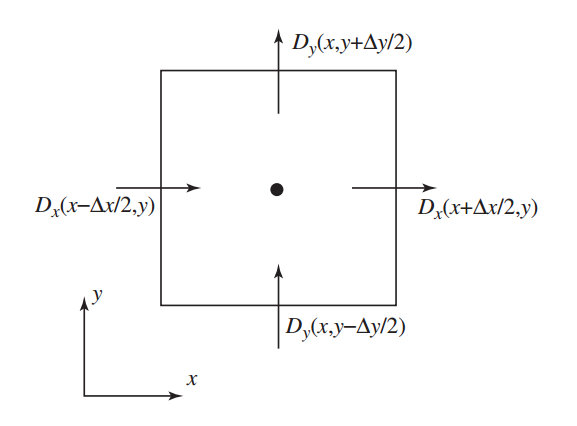
\includegraphics{img/divergence.png} Considerese entonces las
diferencias en el plano xy por ejemplo para la densidad del flujo
eléctrico \(D\)

\begin{equation}
\frac{\partial D_x}{\partial x} + \frac{\partial D_y}{\partial y} \approx \frac{ D_x(x + \frac{\Delta x}{2},y) - D_x(x - \frac{\Delta x}{2},y)}{\Delta x} + \frac{ D_x(x ,y + \frac{\Delta y}{2}) - D_x(x, y- \frac{\Delta y}{2})}{\Delta y}
\end{equation}

Si se pone atención en los signos de la expresión anterior se puede
encontrar el sentido del campo vectorial evaluado en los puntos, de modo
que la divergencia es esencialemente la suma sobre los campos en las
caras del rectángulo con los signos denotando flujo hacia adentro
(negativo) y flujo hacia afuera (positivo). Esto tiene un fundamento
importante en el comportamiento del flujo eléctrico en presencia de
carga, en el cual la divergencia del campo representa la fuerza con que
se es atractor o repulsor.

Por otro lado, si se considera el operador de torsión ahora sobre por
ejemplo el campo eléctrico \(E\)

\begin{equation}
\nabla \times E = a_x (\frac{\partial E_z}{\partial y}  - \frac{\partial E_y}{\partial z}) + a_y(\frac{\partial E_x}{\partial z}  - \frac{\partial E_z}{\partial x}) +a_z(\frac{\partial E_y}{\partial x}  - \frac{\partial E_x}{\partial y}) 
\end{equation}

En este caso veamos el comportamiento únicamente de la componente \(z\)
del operador, que está gobernada por el plano xy.

\begin{equation}
\frac{\partial E_y}{\partial x}  - \frac{\partial E_x}{\partial y} \approx  \frac{ E_y(x + \frac{\Delta x}{2},y) - E_y(x - \frac{\Delta x}{2},y)}{\Delta x} - \frac{ E_x(x ,y + \frac{\Delta y}{2}) - E_x(x, y- \frac{\Delta y}{2})}{\Delta y}
\end{equation}

De nuevo inspeccionando la fórmula anterior y siendo apoyado en la
representación gráfica que se muestra a continuación se puede observar
que las aproximaciones de diferencias finitas de nuevo están basadas en
los valores del campo en las orillas del rectángulo que rodean el punto
de interés \((x,y)\). No obstante, en este caso son las fuerzas
tangenciales y no las fuerzas normales a los bordes del rectángulo. La
suma del lado derecho tiene un signo positivo cuando la componente
vectorial apunta en dirección contrario a las manecillas del reloj y es
negativa cuando va en el sentido del reloj. En términos físicos, cuando
la suma es positiva el campo electrico tiene a empujar carga positiva en
la dirección contraria de las manecillas.

\begin{figure}
\centering
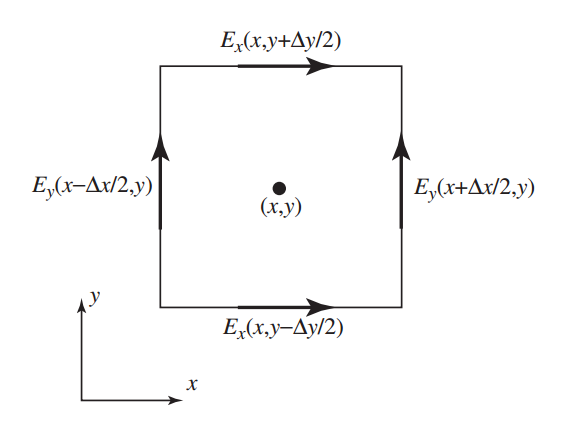
\includegraphics{img/curl.png}
\caption{Aproximación Discreta de la divergencia sobre el plano}
\end{figure}

\subsection{Condición de Estabilidad}\label{condicion-de-estabilidad}

Courant (1928) tuvo un desarrollo importante para establecer las
condiciones de estabilidad para el esquema de muestreo temporal para la
aproximación de las derivadas en el esquema de diferencias finitas
cuando se requiere resolver un sistema de ecuaciones clásico para la
interacción entre campos eléctricos y campos magnéticos. La derivación
de esta cota para la estabilidad en términos de convergencia cuadrática
es muy similar a la que realiza Euler para el caso del método de
aproximación para ecuaciones diferenciales ordinarias.

\begin{equation}
\Delta x \leq \frac{\lambda}{10}; \text{ Estabilidad si }  \Delta t \leq  \frac{\Delta x}{c \sqrt{\alpha}}
\end{equation}

donde \(\alpha\) varía dependiendo si es un espacio \(\alpha\)
dimensional. Es decir \(\alpha=1\) en el caso unidimensional,
\(\alpha=2\) en 2D y \(\alpha=3\) en el caso de 3 dimensiones.

\subsection{Modelo Físico}\label{modelo-fisico}

Cuando se consideran campos que son dinámicos, es decir se mueven a lo
largo del tiempo es importante formular el problema pensando en qué debe
sucedes cuando una carga puntual se mueve? Se sabe que cuando una carga
está en movimiento esto origina un campo magnético, pero si la carga se
mueve su campo eléctrico asociado también debe cambiar. Por lo mismo se
dice que cuando un sistema varía en el tiempo entonces los campos
magnéticos y los campos eléctricos están acoplados. Uno de los grandes
reconocimientos que lleva a cabo Maxwell es que se debe considerar que
la densidad de carga puede cambiar en el tiempo de modo que el decidió
incorporar la derivada temporal de la densidad del flujo eléctrico para
poder obtener un modelo más general que no solo aplicara a campos que no
cambian en el tiempo.

\begin{equation}
\nabla \times H = J + \frac{\partial D}{\partial t}
\end{equation}

Los términos \(J\) y \(\frac{\partial D}{\partial t}\) suelen ser
identificados con la corriente conductiva y la corriente de
dezplazamiento respectivamente y es comunmente conocida como la Ley de
Ampere.

Si se considera el cambio en el potencial eléctrico sobre alguna
trayectoria es decir la fuera electromotriz ejercida por el campo, en
particular sobre una trayectoria cerrada se escribe como la integral de
linea del producto punto del vector de velocidad con el campo E y al
hacer uso del teorema de stokes se tiene que es igual al cambio sobre la
densidad del flujo magnetico B sobre la superficie que encierra dicha
trayectoria, de donde se sigue que

\begin{equation}
\nabla \times E = - \frac{\partial B}{\partial t}
\end{equation}

la cual es conocida como la Ley de Faraday.

Las ecuaciones de Maxwell están constituidas por un conjunto de
ecuaciones diferenciales parciales, las cuales junto con una ley de
fuerza de Lorentz, conforman el fundamento del electromagnetismo y
óptica clásicos así como de los circuitos eléctricos. Las ecuaciones son
nombradas en honor al físico y matemático James Clerk Maxwell, quien
entre 1861 y 1862 publicó las ecuaciones así como una proposición de que
la luz es un fenómeno electromagnético. En particular en un medio
isotrópico se tiene que las ecuaciones toman la forma siguiente (en MKS)

\begin{eqnarray}
\frac{\partial \mathbf{B}}{\partial t} + \nabla \times \mathbf{E} &=0  \\
\frac{\partial \mathbf{D}}{\partial t} - \nabla \times \mathbf{H} &=\mathbf{J}  \\
\mathbf{B} &= \mu \mathbf{H} \\
\mathbf{D} &= \epsilon \mathbf{E} 
\end{eqnarray}

En las cuales se asume que \(\mathbf{J}\), \(\mu\) \(\epsilon\) son
funciones del espacio tiempo conocidas. Recordar que \(H\) e sun campo
magnético auxilar que representa como un campo magnético B influye sobre
la organización de los dipolos magnéicos es un medio determinado,
incluyendo la migración dipolar y la reorientación dipolar magnética,
con \(\mu\) representa la permeabilidad. En el caso en el que el medio
es isotropico (es decir igual en todas las direcciones) entonces \(\mu\)
es un escalar. Cuando el medio es anisotrópico \(\mu\) resulta ser un
tensor de segundo rango. En general la permeabilidad es la medida en que
un material puede soportar la formación del campo magnético en si mismo,
es decir es el grado de magnetización de que un material obtiene en
respuesta a la aplicación de un campo magnético. Está medida en henries
por metro \(H/m\) o bien newtons por ampere al cuadrado \(N/A^2\)

\begin{figure}[htp]
\centering
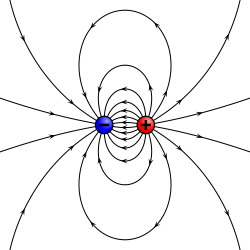
\includegraphics[width=.3\textwidth]{img/dipole_electric.svg.png}
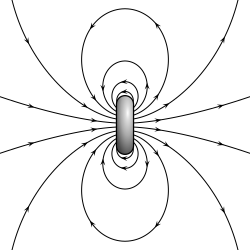
\includegraphics[width=.3\textwidth]{img/dipole_magnetic.svg.png}
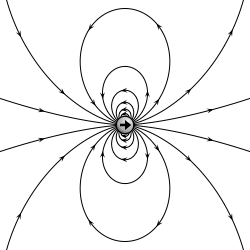
\includegraphics[width=.3\textwidth]{img/dipole_point.svg.png}
\caption{Campos para un par de polos eléctricos, un dipolo magnético y un dipolo general (límite cuando la distancia entre polos tiende a cero)}
\end{figure}

\subsection{Discretizacion del
problema}\label{discretizacion-del-problema}

En términos de un sistema de coordenadas rectangulares las Leyes de
Faraday y Ampere, son equivalentes a

\begin{eqnarray}
- \frac{\partial \mathbf{B}_x}{\partial t} &= \frac{\partial \mathbf{E}_z}{\partial y} - \frac{\partial \mathbf{E}_y}{\partial z} \\
- \frac{\partial \mathbf{B}_y}{\partial t} &= \frac{\partial \mathbf{E}_x}{\partial z} - \frac{\partial \mathbf{E}_z}{\partial x} \\
\frac{\partial \mathbf{B}_z}{\partial t} &= \frac{\partial \mathbf{E}_x}{\partial y} - \frac{\partial \mathbf{E}_y}{\partial x} \\
\frac{\partial \mathbf{D}_x}{\partial t} &= \frac{\partial \mathbf{H}_z}{\partial y} - \frac{\partial \mathbf{H}_y}{\partial z} -\mathbf{J}_x \\
\frac{\partial \mathbf{D}_y}{\partial t} &= \frac{\partial \mathbf{H}_x}{\partial z} - \frac{\partial \mathbf{H}_z}{\partial x} -\mathbf{J}_y \\
\frac{\partial \mathbf{D}_z}{\partial t} &= \frac{\partial \mathbf{H}_y}{\partial x} - \frac{\partial \mathbf{H}_x}{\partial y} -\mathbf{J}_z \\
\end{eqnarray}

En el caso de discretización tridimensional se denota a un punto de la
malla

\begin{equation}
(i,j.k) = (i\Delta x, j\Delta y, k\Delta z) y 
\end{equation}

y para cualquier función del espacio tiempo se define

\begin{equation}
F(i\Delta x, j\Delta y, k\Delta z, n\Delta t) = F^n(i,j,k)
\end{equation}

\subsubsection{Sistemas de Ecuaciones}\label{sistemas-de-ecuaciones}

Un conjunto de ecuaciones de diferencias finitas para el sistema arriba
descrito para el caso de condiciones de frontera de conductividad
perfecta son

\begin{equation}
\frac{B_x^{n+\frac{1}{2}}(i,j+\frac{1}{2},k+\frac{1}{2}) - B_x^{n-\frac{1}{2}}(i,j+\frac{1}{2},k+\frac{1}{2})}{\Delta t} = \frac{E_y^n(i,j+\frac{1}{2},k+1) - E_y^n(i,j+\frac{1}{2},k)}{\Delta z} - \frac{E_z^n(i,j+1,k+\frac{1}{2}) - E_z^n(i,j,k+\frac{1}{2})}{\Delta y}
\end{equation}

Las correspondientes discretizaciones para 2b y 2c son analogas

\begin{equation}
\frac{D_x^{n}(i+\frac{1}{2},j,k) - D_x^{n-1}(i+\frac{1}{2},j,k)}{\Delta t} = \frac{H_z^{n-\frac{1}{2}}(i+\frac{1}{2},j+\frac{1}{2},k) - H_z^{n-\frac{1}{2}}(i+\frac{1}{2},j-\frac{1}{2},k)}{\Delta y} - \frac{H_y^{n-\frac{1}{2}}(i+\frac{1}{2},j,k+\frac{1}{2}) - H_y^{n-\frac{1}{2}}(i+\frac{1}{2},j,k-\frac{1}{2})}{\Delta z} + J_x^{n-\frac{1}{2}}(i+\frac{1}{2},j,k)
\end{equation}

\paragraph{Condiciones de Frontera}\label{condiciones-de-frontera}

Las condiciones de frontera para una superficie de conductividad
perfecta se traduce en que las componentes tangenciales del campo
eléctrico se desvanecen. Esta condición también implica que las
componentes normales del campo mágnetico se desvanecen en el superficie.
La superficie de conducción será aproximada a través de una colección de
superficies de cubos cuyas aristas y lados son paralelos a los ejes
coordenados como se muestra en la figura.

\begin{figure}
\centering
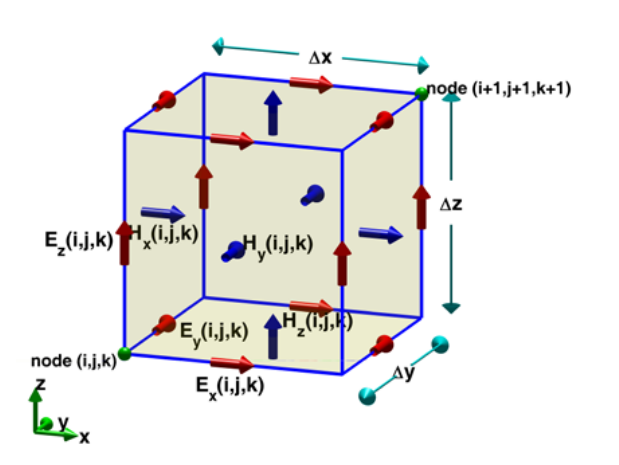
\includegraphics{img/yee_cell.png}
\caption{Celda de Yee: Unidad del Dominio Computacional}
\end{figure}

El espacio de la malla debe ser tal que un incremento el campo
electromagnetico no cambie significativamente. Esto significa ue para
tener resultados plausibles la dimensión lineal de la malla debe ser una
fracción de la longitud de onda. En este caso
\(\Delta x = \Delta y = \Delta z\) . Para estabilidad computacional es
necesario satisfacer una relaci entre los incrementos espaciales y los
temporales. Cuando \(\epsilon\) y \(\mu\) son variables, un criterio
rigurosos es dificil de obtener, pero en el caso en que son constantes

\begin{equation}
\sqrt{ (\Delta x)^2+(\Delta y)^2+(\Delta z)^2} > c\Delta t = \sqrt{ \frac{1}{\mu \epsilon}}\Delta t
\end{equation}

donde \(c\) es la velocidad de la luz. Este requerimiento pone
restricciones sobre \(\Delta t\) dados los incrementos espaciales.

El algortimo fue propuesto por Kane Yee en {[}1966{]} en el cual se usan
diferencias centradas de segundo orden y puede ser resumido de la
siguiente forma

\begin{itemize}
\item Se reemplazan todas las derivadas de las leyes de Ampere y Faraday por diferencias finitas. Se discretiza el espacio y tiempo de modo que los campos eléctrico y magnético are staggered tanto en tiempo como en espacio. 
\item Se resuelve el sistema de diferencias finitas para obtener ecuaciones de actualización que expresan los campos futuros desconocidos en términos de campos pasados conocidos. 
\item Se evalúan los campos magnéticos un paso temporal hacia el futuro de modo que sean conocidos
\item Se evalúan los campos eléctricos un paso temporal hacia el futuro de modo que se vuelven conocidos
\item Se repite los pasos previos hasta que se obtenga la duración deseada. 
\end{itemize}

En el modelo discretizado se tiene que las componentes eléctricas son
tangenciales a la celda de Yee mientras que las componentes magnéticas
son ortogonales a la caras de la celda.

En un ejemplo se puede considerar \(J \equiv 0\) y tomar \(\mu\) y
\(\epsilon\) constantes de modo que sea sencillo interpretar los
conceptos fundamentales de una onda sencilla que se dispersa. De hecho
se puede tener una descomposición importante si se realiza un cambio de
coordenadas. En particular se tiene que en coordenadas cilindrícas
cualquier campo electromagnético se puede descomponer en dos campos
básicos: el campo transversal eléctrico (TE) y el campo transversal
magnético (TM) en el caso que \(\epsilon\) y \(\mu\) son constantes

\begin{figure}
\centering
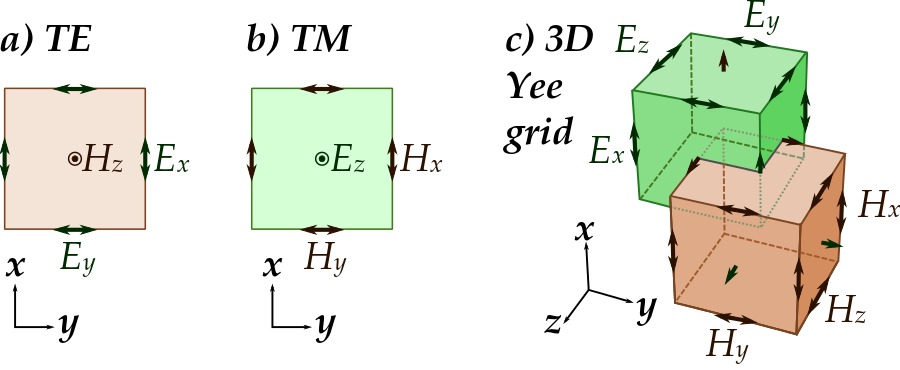
\includegraphics{img/yee_2d_3d.png}
\caption{Descomposición en campos transversales}
\end{figure}

Es importante notar que los cubos `aproximan' el fenómeno en cuatro
dimensiones, es decir la evolución del campo. En términos de las
aproximaciones del cálculo dierencial, se hace uso de aproximaciones
tridimensionales sucesivas en el dominio temporal para aproximar los
valores de la función que satisface el sistema de ecuaciones que dicta
la dinámica del campo electromagnético. En particular el sistema de
diferencias finitas encontrado explícitamente de las aproximaciones de
segundo orden, realiza el efecto que tiene un campo sobre el otro a lo
largo del tiempo, creando así un mecanismo de actualización sobre el
conjunto discreto que es la malla tridimensional.

\subsection{Arquitectura Computacional:
CUDA}\label{arquitectura-computacional-cuda}

Las unidades de procesamiento grafico (GPU) están adecuadas
especialmente para atacar problemas que pueden ser expresadas como
computo en paralelo, esto es el mismo programa es ejecutado en muchos
elementos en paralelo. Por otro lado el algoritmo de diferencias finitas
en el dominio temporal (FDTD) es ese tipo de algoritmos que ejecuta el
mismo cálculo en todas las componentes del campo tridimensional en todas
las celdas del dominio computacional.

CUDA C extiende el lenguaje de programación C al permitir que el
programador defina funciones de C, llamadas kernels, que son aquellas
que ejecutan N veces en paralelo por N diferentes threads. Cada thread
que ejecuta el kernel tiene un \texttt{threadId} único que es posible de
acceder desde el kernel a través de la variable \texttt{threadIdx}, que
por conveniencia es un vector de 3 componentes, de modo que los threads
pueden ser identificados por un indice de 1,2 o 3 dimensiones formando
un bloque de threads que puede ser de 1,2 o 3 dimensiones.

Dado que el kernel se ejecuta en bloques que tienen la misma forma, el
numero total de threads es igual al numero de threads por bloque
multiplicado por el número de bloques. Los múltiples bloques pueden
estar organizados en una malla uni o bi dimensional. Cada bloque en la
malla está identificado con un indice uni o bidimensional que es
accesible desde el kernel a través de la variable \texttt{blockIdx}.

\subsubsection{Espacios de Memoria}\label{espacios-de-memoria}

Los threads de CUDA pueden acceder a los datos desde múltples espacios
de memoria durante su ejecución. Cada thread tiene una memoria local
privada y una memoria compartida que es visible para todoss los threads
del bloque y con la misma duración que el bloque. Todos los threads
tienen acceso a la misma memoria global, la cual es el espacio principal
de memoria en el device en la que se almacenan los datos.

\begin{figure}
\centering
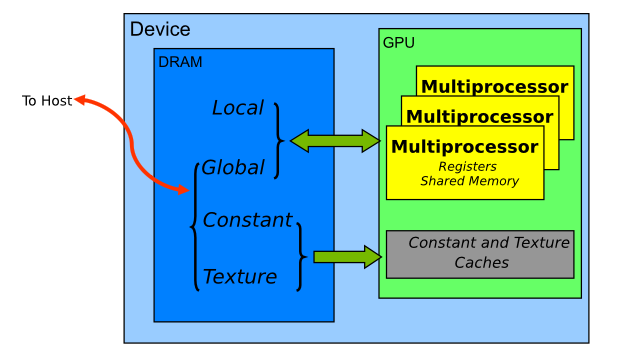
\includegraphics{img/memoria_cuda.png}
\caption{Espacios de Memoria en el Device}
\end{figure}

Acceso a la memoria global es muy limitada y se convierte en el
principal cuello de botella en la ejecución del kernel. Por otro lado la
memoria compartida es mucho más rápida de acceder pero en términos de
tamaño es muy limitada. No obstante, provee de los medios para
reutilizar datos y mejorar la eficiencia del kernel.

Los espacios de memoria constante y textura son dos espacios adicionales
de lectura limitadas en tamaño y accedibles por todos los threads
durante toda la aplicación.

El kernel ejecuta en una unidad de procesamiento gráfico a la que es
referida como el \emph{device} y el resto del programa se ejecuta en la
unidad de procesamiento central y es referida como \emph{host}

\subsubsection{Estrategias de
optimización}\label{estrategias-de-optimizacion}

En los manuales de programación de CUDA se exponen mejores prácticas,
las cuales fungen como recomendaciones para optimizar las
implementaciones de algoritmos en general. Entre las más importantes
están

\begin{itemize}
\item
  Estructurar los algoritmos de forma que se exhiba el paralelismo en
  los cálculos tanto como sea posible
\item
  Una vez que el algoritmo tiene dicha estructura, es necesario un mapeo
  hacia el hardware tan eficiente como sea posible
\item
  Asegurarse que los accesos a memoria global sean de tipo coalescente
  siempre que sea posible.
  \footnote{Coalescencia: Es la propiedad de las cosas para unirse o fundirse. En términos computacionales fue una novedad de los GPUS, ya que tienen la capacidad de fusionar bloques adyacentes de memoria para llenar las brechas ocasionadas por la memoria desalojada}
\item
  Minimizar el uso de memoria global y preferentemente usar en su lugar
  memoria compartida
\item
  Usar memoria compartida para evitar transferencias redundantes desde
  la memoria global
\item
  Reducir la latencia que surge de las dependencias con el register,
  esto es tiempo de transferencia entre memoria
\item
  Usar múltiplos de 32 para el número de threads por bloque, ya que
  estro permite eficiencia óptima en computo y facilita la coalescencia
\end{itemize}

Más en
\url{http://docs.nvidia.com/cuda/cuda-c-best-practices-guide/#memory-optimizations}

\begin{figure}
\centering
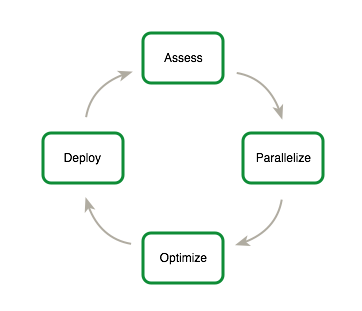
\includegraphics{img/best_cuda.png}
\caption{Ciclo de diseño para aceleración GPU}
\end{figure}

\section{Implementación de FDTD en
GPU}\label{implementacion-de-fdtd-en-gpu}

La formulación considerada en CUDA está fundamentada en actualizar las
ecuaciones para propiedades anisotropicas de materiales en las se que se
incluyen permisividad, permeabilidad y conductividades eléctrica y
magnética. El dominio para el problema FDTD es una celda, referida en la
literatura como la celda de Yee, como se muestra a continuación.

\subsection{Construccion del Kernel}\label{construccion-del-kernel}

En cada iteración temporal del ciclo de FDTD se calculan tres valores
para el campo magnético en cada celda del dominio computacional de forma
simultánea con base en los valores pasados del campo eléctrico y
asimismo se calculan tres valores que actualizan las componentes del
campo eléctrico de forma simultánea. Dado que los cálculos para cada
celda pueden ser realizados de forma independiente de las demás celdas,
se puede diseñar una implementación que asigne el cálculo de cada celda
a thread independientes y que así esta alcance un nivel alto de
paralelización.

En CUDA cada bloque tiene un máximo posible de 512 threads, los cuales
pueden ser organizados en 1, 2 o 3 dimensiones. Por lo tanto una
subsección del problema en un espacio tridimensional puede ser
naturalmente mapeado a un bloque de threads tridimensional. Sin embargo,
los bloques sólo pueden ser organizados en mallas de forma
unidimensional o bidimensional, por lo que el dominio tridimensional
entero del algoritmo de diferencias finitas en el dominio temporal no
puede ser mapeado naturalmente a una malla uni o bi dimensional, por lo
que se debe utilizar un mapeo alternativo para el dominio del algoritmo
FDTD

\subsubsection{Acceso a Memoria Global
Coalesced}\label{acceso-a-memoria-global-coalesced}

Las instrucciones de memoria incluyen cualquier instrucción que lee
desde o escribe a cualquier memoria compartida, local o global. Cuado se
accede a la memoria local o global hay entre 400 y 600 clock cycles de
memory latency.

En ciertas ocasiones está latencia puede ser escondida por el scheduler
de threads si existen instrucciones arimeticas que puedes ser
consideradas mientras se espera por el acceso a la memoria global. La
mala noticia es que en el caso del FDTD las operaciones están dominadas
por accesos a memoria más que por instrucciones aritméticas, por lo que
el acceso ineficiente a memoria resulta el principal cuello de botella
para los GPUS.

El ancho de banda de memoria global es usadata casi eficientemente
cuando los accesos simultaneos por los threads en un half-warp (durante
la ejecucion de una instrucción de escritura o lectura) puede ser
coalescida en una sola transacción de memoria de 32 64 o 128 bytes.

\subsubsection{Acceso a Memoria
Compartida}\label{acceso-a-memoria-compartida}

El acceso a memoria compartida es mucho más rápida que la memoria local
o global debido a que es una memoria on-chip. Aquellos parametros que
residan en el espacio de memoria compartida de un bloque de threads
tienen la misma duración que el bloque y son accedibles por todos
losthreads del bloque. Por lo que si el kernel utilizará frecuentemente
bloques de información de la memoria global es mejor cargar los datos en
la memoria compartida para que exista reciclado de datos.

En particular la memoria compartida es muy útil en el caso que lso
threads deben acceder a datos `desalineados' (unaligned), por ejemplo
para calcular \(H_y(i,j,k)\), un thread es mapeado a la celda
\((i,j,k)\) necesita \(E_x\) y \(E_z\) en \((i,j,k)\) así como en
\(E_x\) en \((i,j,k+1)\) y \(E_z(i+1,j,k)\). En un caso se tiene que el
acceso posee coalescencia sobre \((i,j+1,k)\) y \((i,j,k+1)\), no
obstante \((i+1,j,k)\) no lo está y si es necesario un acceso a una
celda vecina que no está en modo de coalescencia \(E_z(i+1,j,k)\) para
\(H_y(i,j,k)\) y \(E_y(i+1,j,k)\) para \(H_z(i,j,k)\) entonces la
memoria compartida se puede utilizar para cargar el bloque de datos
mapeados a un bloque de threads y el campo vecino es accedido a través
de memoria compartida.En este punto uno necesita utilizar la
sincronización de los thredas en un bloque de modo que todos los datos
necearios estén cargadps en memoria compartida antes de que se usen por
sus threads vecinos.

Aunque los accesos que no son coalsced pueden ser eliminados usando
memoria compartida existe un problema cuando se accede a la información
de celdas vecinas a través de la memoria compartida. Cuando se carga la
memoria compartida cada thread copia un elemetod de la memoria global a
la memoria compartida, si el thread de la frontera del bloque desea
acceder a la informacion de la celda vecina estos datos no estarán
disponibles si no están cargados en la memoria compartida. Por lo tanto
es necesario cargar otro conjunto de datos que inluye los datos de las
celdas vecinas a la memoria compartida.

La asignación de espacio se extienda por 16 y en algunos threads del
bloque son utilizados para copiar datos de la memoria global a esta
extensión de la memoria compartida. Así las transferencias de datos
desde y hacia la memoria global deben ser evitadas tanto com osea
posible. en algunos casos es mejor recalcular que volver a leer de la
memoria global. En otras palabras si hay datos que ya han sido
transferidos desde la memoria global ddeben ser utilizados tantas veces
sea posible.

\begin{table}[htbp]
\centering
\caption{Características de los Espacios de Memoria}
\begin{tabular}{l|l|l|l|l|l}
Memory & Location on/off chip & Cached & Access & Scope & Lifetime \\
\hline
Register & On & n/a & R/W & 1 thread & Thread \\
Local & Off & Yes & R/W & 1 thread & Thread \\
Shared & On & n/a & R/W & All threads in block & Block \\
Global & Off & Yes & R/W & All threads + host & Host allocation \\
Constant & Off & Yes & R & All threads + host & Host allocation \\
Texture & Off & Yes & R & All threads + host & Host allocation
\end{tabular}
\end{table}

\subsection{Código BASE}\label{codigo-base}

A continuación llevamos a cabo la descripción del código de los archivos
integrados en el ejemplo del método de diferencias finitas en el dominio
temporal. En general se tienen dos carpetas, una \emph{inc} y otra
\emph{src} que contienen los headers a incluir y el código fuente que
compila las rutinas principales, respectivamente.

\begin{itemize}
\tightlist
\item
  \texttt{*inc*}

  \begin{itemize}
  \tightlist
  \item
    FDTD3d.h
  \item
    FDTD3dGPU.h
  \item
    FDTD3dGPUKernel.cuh
  \item
    FDTD3dReference.h
  \end{itemize}
\item
  \texttt{*src*}

  \begin{itemize}
  \tightlist
  \item
    FDTD3d.cpp
  \item
    FDTD3dGPU.cu
  \item
    FDTD3dReference.cpp
  \end{itemize}
\end{itemize}

Junto con estos archivos se encuentran el archivo \texttt{Makefile} que
se encarga de llevar a cabo el proceso de compilación de los archivos
fuente. * FDTD3d.txt * Makefile * NsightEclipse.xml * readme.txt

\paragraph{INC}\label{inc}

En la carpeta \textbf{inc} incluimos todos los archivos a incluir en el
codigo de C. Principalmente \emph{header files} tanto para el caso
paralelo como para el no-paralelo. Estos archivos despues seran
``incluidos'' \texttt{\#include} en las partes ``centrales'' del codigo
de C.

\textbf{FDTD3d.h}

\emph{Header file.} Definimos las variables a usar para el caso no
paralelo.

\begin{Shaded}
\begin{Highlighting}[]
\PreprocessorTok{#ifndef _FDTD3D_H_}
\PreprocessorTok{#define _FDTD3D_H_}
\end{Highlighting}
\end{Shaded}

Definimos las dimensiones minimas y maximas de las matrices. Estos se
pueden ajustar pero cuando son operaciones de grandes dimensiones puede
tomar muchisimo tiempo en correr.

\begin{Shaded}
\begin{Highlighting}[]
\PreprocessorTok{#define k_dim_min           96}
\PreprocessorTok{#define k_dim_max           376}
\PreprocessorTok{#define k_dim_qa            248}
\end{Highlighting}
\end{Shaded}

Definimos el radio que usara el kernel, lo definimos como 4 ya que se
necesita una constante. Si se ajusta este variable se debe de hacer su
respectivo ajuste en el kernel.

\begin{Shaded}
\begin{Highlighting}[]
\PreprocessorTok{#define k_radius_min        4}
\PreprocessorTok{#define k_radius_max        4}
\PreprocessorTok{#define k_radius_default    4}
\end{Highlighting}
\end{Shaded}

\begin{Shaded}
\begin{Highlighting}[]
\PreprocessorTok{#define k_timesteps_min     1}
\PreprocessorTok{#define k_timesteps_max     10}
\PreprocessorTok{#define k_timesteps_default 5}
\end{Highlighting}
\end{Shaded}

\textbf{FDTD3dGPU.h}

\emph{Header filea} En esta parte definimos el codigo para el caso
paralelo.

\begin{Shaded}
\begin{Highlighting}[]
\PreprocessorTok{#ifndef _FDTD3DGPU_H_}
\PreprocessorTok{#define _FDTD3DGPU_H_}
\end{Highlighting}
\end{Shaded}

\begin{Shaded}
\begin{Highlighting}[]
\PreprocessorTok{#include }\ImportTok{<cstddef>}
\PreprocessorTok{#if defined(WIN32) || defined(_WIN32) || defined(WIN64) || defined(_WIN64) && defined(_MSC_VER)}
\KeywordTok{typedef} \DataTypeTok{unsigned} \NormalTok{__int64 }\DataTypeTok{memsize_t}\NormalTok{;}
\PreprocessorTok{#else}
\PreprocessorTok{#include }\ImportTok{<stdint.h>}
\KeywordTok{typedef} \DataTypeTok{uint64_t} \DataTypeTok{memsize_t}\NormalTok{;}
\PreprocessorTok{#endif}
\end{Highlighting}
\end{Shaded}

\begin{Shaded}
\begin{Highlighting}[]
\PreprocessorTok{#define k_blockDimX    32}
\PreprocessorTok{#define k_blockDimMaxY 16}
\PreprocessorTok{#define k_blockSizeMin 128}
\PreprocessorTok{#define k_blockSizeMax (k_blockDimX * k_blockDimMaxY)}
\end{Highlighting}
\end{Shaded}

Definimos todas las variables usadas para el caso paralelo. Como el
radio, las 3 dimensiones a usar, etc.

\begin{Shaded}
\begin{Highlighting}[]
\DataTypeTok{bool} \NormalTok{getTargetDeviceGlobalMemSize(}\DataTypeTok{memsize_t} \NormalTok{*result, }\AttributeTok{const} \DataTypeTok{int} \NormalTok{argc, }\AttributeTok{const} \DataTypeTok{char} \NormalTok{**argv);}
\DataTypeTok{bool} \NormalTok{fdtdGPU(}\DataTypeTok{float} \NormalTok{*output, }\AttributeTok{const} \DataTypeTok{float} \NormalTok{*input, }\AttributeTok{const} \DataTypeTok{float} \NormalTok{*coeff, }\AttributeTok{const} \DataTypeTok{int} \NormalTok{dimx, }\AttributeTok{const} \DataTypeTok{int} \NormalTok{dimy, }\AttributeTok{const} \DataTypeTok{int} \NormalTok{dimz, }\AttributeTok{const} \DataTypeTok{int} \NormalTok{radius, }\AttributeTok{const} \DataTypeTok{int} \NormalTok{timesteps, }\AttributeTok{const} \DataTypeTok{int} \NormalTok{argc, }\AttributeTok{const} \DataTypeTok{char} \NormalTok{**argv);}
\end{Highlighting}
\end{Shaded}

\textbf{FDTD3dGPUKernel.cuh}

\emph{Header file de cuda.} Definimos las variables a usar en el kernel
de CUDA:

\textbf{FDTD3dGPUReference.h}

\emph{Header file.} Declaramos todas las variables a usar en partes
posteriores del codigo.

\begin{Shaded}
\begin{Highlighting}[]
\DataTypeTok{void} \NormalTok{generateRandomData(}\DataTypeTok{float} \NormalTok{*data, }\AttributeTok{const} \DataTypeTok{int} \NormalTok{dimx, }\AttributeTok{const} \DataTypeTok{int} \NormalTok{dimy, }\AttributeTok{const} \DataTypeTok{int} \NormalTok{dimz, }\AttributeTok{const} \DataTypeTok{float} \NormalTok{lowerBound, }\AttributeTok{const} \DataTypeTok{float} \NormalTok{upperBound);}
\DataTypeTok{void} \NormalTok{generatePatternData(}\DataTypeTok{float} \NormalTok{*data, }\AttributeTok{const} \DataTypeTok{int} \NormalTok{dimx, }\AttributeTok{const} \DataTypeTok{int} \NormalTok{dimy, }\AttributeTok{const} \DataTypeTok{int} \NormalTok{dimz, }\AttributeTok{const} \DataTypeTok{float} \NormalTok{lowerBound, }\AttributeTok{const} \DataTypeTok{float} \NormalTok{upperBound);}
\DataTypeTok{bool} \NormalTok{fdtdReference(}\DataTypeTok{float} \NormalTok{*output, }\AttributeTok{const} \DataTypeTok{float} \NormalTok{*input, }\AttributeTok{const} \DataTypeTok{float} \NormalTok{*coeff, }\AttributeTok{const} \DataTypeTok{int} \NormalTok{dimx, }\AttributeTok{const} \DataTypeTok{int} \NormalTok{dimy, }\AttributeTok{const} \DataTypeTok{int} \NormalTok{dimz, }\AttributeTok{const} \DataTypeTok{int} \NormalTok{radius, }\AttributeTok{const} \DataTypeTok{int} \NormalTok{timesteps);}
\DataTypeTok{bool} \NormalTok{compareData(}\AttributeTok{const} \DataTypeTok{float} \NormalTok{*output, }\AttributeTok{const} \DataTypeTok{float} \NormalTok{*reference, }\AttributeTok{const} \DataTypeTok{int} \NormalTok{dimx, }\AttributeTok{const} \DataTypeTok{int} \NormalTok{dimy, }\AttributeTok{const} \DataTypeTok{int} \NormalTok{dimz, }\AttributeTok{const} \DataTypeTok{int} \NormalTok{radius, }\AttributeTok{const} \DataTypeTok{float} \NormalTok{tolerance=}\FloatTok{0.}\ErrorTok{0001f}\NormalTok{);}
\end{Highlighting}
\end{Shaded}

\paragraph{SRC}\label{src}

En esta parte incluimos el \emph{source code.} Esta es la parte
``central'' del programa.

\textbf{FDTD3d.cpp}

*Codigo para implemententacion de FDTD. No-paralelo.

\textbf{FDTD3dGPU.cpp}

*Codigo para implemententacion de FDTD usando GPU. Modo paralelo.

\textbf{FDTD3dGPUReference.cpp}

Definicion de variables a usar en el codigo de paralelo.

\paragraph{Makefile}\label{makefile}

Makefile para la compilacion del program. Incluye las partes del codigo
de CUDA.

\paragraph{NsightEclipse.xml}\label{nsighteclipse.xml}

\emph{Project file.} Contiene la informacion acerca del proyecto.

\subsection{Desempeño del código}\label{desempeno-del-codigo}

Fue examinado como una función del tamaño en el algoritmo \ldots{} como
un mapeo xy xyz? El análisis se realizó con una tarjeta
\href{http://www.geforce.com/hardware/notebook-gpus/geforce-gtx-960m/specifications}{NVIDIA
GEForce GTX 960M} que tiene 640 CUDA cores en una máquina con
Ubuntu-Linux 64 bit. \ldots{} Dado que se recorrio un dominio de tamaño
cúbico en el problema de diferencias finitas en el tiempo, el numero de
millón de celdas por segundo (NMCPS) es calculado como medida de
desempeño del programa de CUDA

\begin{equation}
NMCPS = \frac(NMCPS){n_{steps} \times N_x \times N_y \times N_z}{t_s}\times 10^{-6}
\end{equation}

donde \(n_{steps}\) es el número de pasos que itera el progama, t\_s el
total de tiempo en segundos.

Determinación del número óptimo de threads CUDA Visual Profiler, las
funciones del kernel que actualizan las componentes de los campos
eléctrico y magnético son ejecutados usando diferentes numeros de
threads por bloque, en este caso 8 Millones = \(200^3\)

\subsection{Resultados / Analisis de Error Numerico
?}\label{resultados-analisis-de-error-numerico}

\section{Infraestructura de Instancias con CUDA en
Amazon}\label{infraestructura-de-instancias-con-cuda-en-amazon}

Para la implementacion del problema, usaremos una instancia EC2 de
Amazon AWS de tipo G2. Estas instancias cuentan con 1,536 cores de CUDA
para paralelizar, asi como un Intel Xeon E5-2670.

La implementacion de FDTD suele ser demasiado costosa
computacionalmente, el avance en el uso de tarjeta graficas para
``general purpose programming'' ha permitido que metodos como el FDTD
puedan ser ejecutados en tiempos razonables.

La ``forma'' tipica en la que es implementado un codigo en CUDA es
similar al mostrado en la imagen a continuacion.

\emph{Basic Code Flowchart}

\begin{figure}
\centering
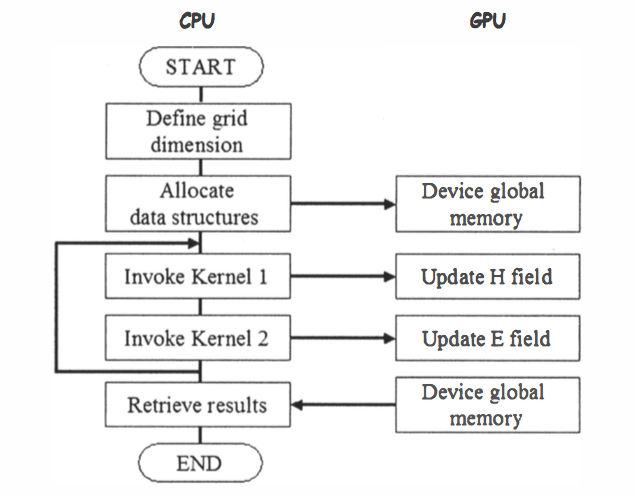
\includegraphics{img/flow.png}
\caption{Diagrama de Comunicación}
\end{figure}

Fuente: D. Danielo,E.Alessandra,T.Luciano,C.Luca, Introduction to GPU
Computing and CUDA Programming: A Case Study on FDTD, Unive ity of
Stellenbosch, June 2010.

El codigo, claro, esta escrito para que pueda ser ejecutado en forma
paralela (Vease archivos de codigo), generalmete de la forma SIMT.
Diversos articulos de la literatura muestran un ganancia en eficiencie
de hasta un 80\% en cuestion de tiempo de ejecucion, este varia un poco
dependiendo de la metrica que se use para medir la eficiencia.

El codigo se planea implementar de tal manera que todos los threads se
utilicen en la maquina de Amazon, asi como eficientar el acceso a
memoria.

\subsection{Docker}\label{docker}

Crearemos un cluster de Docker en una maquina de Amazon. El ejemplo
basico de la integracion de Docker con CUDA se puede observar en la
imagen 1.2.

Para esto, usaremos el Dockerfile oficial de Nvidia, con el ajuste para
correr nuestro codigo.

\begin{figure}
\centering
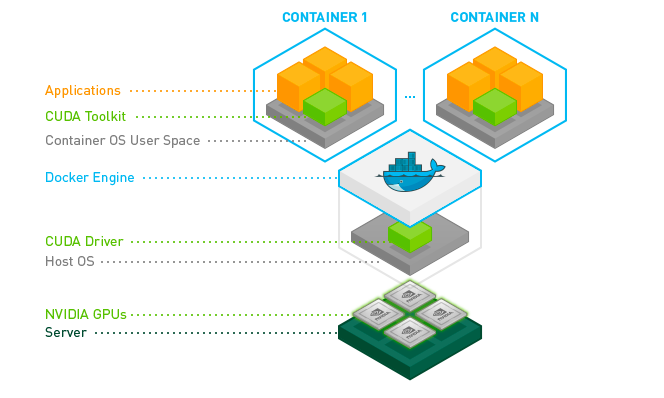
\includegraphics{img/dockercuda.png}
\caption{Arquitectura Fuente: Nvidia Github}
\end{figure}

Los pasos basicos a seguir para una correcta instalacion de CUDA en
Docker y Amazon son:

\begin{itemize}
\tightlist
\item
  Creamos la instancia de Amazon (puede ser via docker-machine)
\item
  Instalamos los drives de Nvidia
\item
  Descargamos la imagen de Docker de NVidia con CUDA o podemos usar una
  propia
\item
  Creamos los contenedores
\item
  Manejamos remotamente con \texttt{nvidia-docker}
\end{itemize}

Esta parte se puede ejecutar corriendo el script de
\texttt{docker-machine.sh}. Tal como se mencionaa arriba, creamos la
isntancia de Amazon de tipo G2, instalaremos los drives de Nvidia asi
como el docker, y despues haremos un deploy via nvidia-docker. El deploy
se puede hacer usando \texttt{deploy.sh}.

\section{Referencias}\label{referencias}

\begin{itemize}
\item
  \href{https://drive.google.com/open?id=0B1GlF2qCvHCXa0JYWHBNcVdmSUk}{Micikevicius,
  P. 3D finite difference computation on GPUs using CUDA. In Proceedings
  of 2nd workshop on general purpose processing on graphics processing
  units pp.~79-84., March, 2009}

  \begin{itemize}
  \item
    \href{https://drive.google.com/open?id=0B1GlF2qCvHCXUlk5NUx1THNxczQ}{V.
    Demir, A.Z. Elsherbeni, ``Compute Unified Device Architecture (CUDA)
    Based Finite- Difference Time-Domain (FDTD) Implementation'', Appl.
    Comput. Electromagn. Soc. J., vol.~25, n. 4, pp.~303-314, April
    2010}
  \item
    \href{https://devblogs.nvidia.com/parallelforall/finite-difference-methods-cuda-cc-part-1/}{Finite
    Difference Methods in CUDA C/C++, Part 1}
  \item
    \href{https://devblogs.nvidia.com/parallelforall/finite-difference-methods-cuda-c-part-2/}{Finite
    Difference Methods in CUDA C/C++, Part 2}
  \item
    \href{https://drive.google.com/open?id=0B1GlF2qCvHCXMkJSWHdhSkFFRFE}{Yee,
    K. Numerical solution of initial boundary value problems involving
    Maxwell's equations in isotropic media. IEEE Transactions on
    antennas and propagation, 14(3), 302-307, 1966}
  \end{itemize}
\end{itemize}


\end{document}
